\documentclass[11pt]{article}

\usepackage[margin=1in]{geometry}
\usepackage{graphicx}
\usepackage{booktabs}
\usepackage{amsmath}
\usepackage{enumitem}
\usepackage{caption}
\usepackage[hidelinks]{hyperref}

\setlength{\parskip}{0.4em}
\setlength{\parindent}{0pt}

\title{\textbf{Fitting Person Detection on a Plain Microcontroller:\\
Architecture and Quantization Tradeoffs for\\
Fixed-Mount CCTV Loitering Detection}}

\author{Akash Reddy K\thanks{Code, raw result JSON, trained weights, and the
figure-generation script for this paper:
\url{https://github.com/akash-reddy-k/edgeAi}. Independent research /
portfolio project.}}

\date{}

\begin{document}

\maketitle

\begin{abstract}
Commercial CCTV analytics (e.g.\ Hikvision AcuSense~\cite{hikvision_acusense},
Ambarella CV7~\cite{ambarella_cv7}) run person detection and event analytics
on purpose-built AI silicon with dedicated neural accelerators. This paper
asks how far equivalent functionality---specifically, loitering detection on
a fixed-mount camera---can be pushed onto a \emph{plain} microcontroller with
no such accelerator. We build a full pipeline: fine-tune YOLOv8n~\cite{yolov8}
for single-class person detection on the ShanghaiTech Campus
dataset~\cite{shanghaitech}, track detections with ByteTrack~\cite{bytetrack},
export to ONNX, and apply static INT8 post-training
quantization~\cite{onnx_quantization}. An analytical ONNX-graph profiler then
measures flash and activation-RAM footprint directly, with no vendor tooling
required. At the stock architecture and a 640$\times$640 input, nothing fits
any plain STM32 part: flash alone overshoots the largest plain part by 50\%.
A six-variant architecture ablation finds that the P5/32 detection pathway,
tuned for objects filling roughly half the frame, accounts for 51.8\% of
parameters and is functionally unused in fixed-mount overhead CCTV; removing
it cuts flash 2.8$\times$---more than INT8 quantization achieved. A trained,
random-init-controlled comparison then shows that reinvesting that budget as
extra width on the two remaining scales beats shrinking all three scales
uniformly, by 3.3 points of mAP50-95. The resulting architecture fits an
STM32H743 at 320$\times$320 with roughly 50\% headroom on both flash and RAM.
We report this as a hardware-feasibility result together with its limits,
including a deliberate negative control (an NPU-equipped part that fits
trivially, by design).
\end{abstract}

\section{Introduction}

Commercial surveillance platforms increasingly ship on-device analytics---
person detection, line-crossing, loitering alerts---on silicon designed for
exactly that job. Hikvision's AcuSense line and Ambarella's CV7 family both
pair a conventional ISP with a dedicated neural processing block, so the
detector runs on hardware built for it~\cite{hikvision_acusense,
ambarella_cv7}. That is a reasonable product decision, but it leaves an
open research question: how much of that capability is actually contingent
on the dedicated accelerator, and how much survives on a plain
microcontroller---the same class of part already soldered onto a huge
installed base of cheap, non-AI fixed-mount cameras?

This paper scopes that question down to one concrete, bounded task:
\textbf{loitering detection on a fixed, overhead-mounted camera.} A person is
detected, assigned a persistent track ID across frames, and an alert fires
once that ID has been continuously present beyond a configurable dwell-time
threshold. This is deliberately narrower than full weakly-supervised video
anomaly detection---the research contribution here is the \emph{compression
and deployment pipeline}, not a new detector or a new anomaly formulation.

\textbf{Contributions.}
\begin{itemize}[leftmargin=1.4em, itemsep=0.2em]
  \item An end-to-end, reproducible pipeline---fine-tune, export, quantize,
  profile, ablate, retrain---with every reported number traceable to a
  committed JSON artifact or training log, and a script
  (\texttt{make\_figures.py}) that regenerates every figure in this paper
  from those artifacts without re-running any measurement.
  \item An analytical flash/activation-RAM profiler that reads an ONNX graph
  directly, with no vendor account or vendor toolchain required, and that
  explicitly models operator fusion (SiLU) and the resolution-dependent
  anchor/stride constants that a naive accounting misses.
  \item A six-variant architecture ablation isolating the P5/32 detection
  pathway as 51.8\% of YOLOv8n's parameters, and showing that removing it is
  a larger, cheaper lever on flash footprint than INT8 quantization.
  \item A trained, random-initialization-controlled comparison between two
  architectures matched to within 5.9\% of the same parameter count---one
  spends the budget on three thinned scales, the other on two full-width
  scales---isolating a genuine architectural effect from a size effect.
  \item A full deployment-feasibility frontier across plain STM32 and ESP32
  parts, stated as an honest negative result at the stock operating point,
  together with the specific architecture and resolution changes that flip
  it positive, and a dedicated-silicon counterexample used as a control.
\end{itemize}

\section{Method}

\subsection{Task and dataset}

All detection and tracking runs against the ShanghaiTech Campus
dataset~\cite{shanghaitech}, a fixed-camera surveillance benchmark. The test
split used here spans 28 scenes (16 containing an annotated anomalous event,
12 normal), split at the \emph{scene} level into 20 training and 8 validation
scenes---no frames from a validation scene appear in training, which rules
out temporal leakage between near-identical adjacent frames.

\textbf{Labelling caveat (read before the Results section).} ShanghaiTech
ships only frame-level anomaly labels (which frame range contains an
anomalous event), not bounding boxes. Object-detector fine-tuning needs
boxes, so training and validation labels were generated by running a
COCO-pretrained~\cite{coco} YOLOv8n over every frame and persisting its
person detections as pseudo-labels. The model was then fine-tuned, and later
ablated, against labels produced by a close relative of itself. This means
every mAP figure in this paper that is computed against those pseudo-labels
measures \emph{how faithfully a model reproduces the base model's own
predictions on campus footage}, not ground-truth detection accuracy, and the
absolute value is inflated. This caveat is stated again, explicitly, in
Section~\ref{sec:limitations}; it governs how every accuracy number in
Section~\ref{sec:results} should be read.

One measurement in this paper is \emph{not} subject to that caveat: a
separate sanity check (Section~\ref{sec:baseline-check}) scores the stock,
COCO-pretrained model's detection rate against ShanghaiTech's real,
human-authored frame-level anomaly labels---an independent signal that was
never used to produce or validate any model weights.

\subsection{Baseline fine-tuning}

A COCO-pretrained YOLOv8n~\cite{yolov8} is fine-tuned for 20 epochs as a
single-class (\texttt{person}) detector on the pseudo-labelled training
split, using Ultralytics' default rectangular batching. This run is the
source of the fine-tuned weights used throughout; its own held-out mAP50 is
not separately reported here because the fairness-controlled, three-way
comparison in Section~\ref{sec:quant-results} supersedes it (see the note on
rectangular vs.\ square batching below).

\subsection{Post-training INT8 quantization}

The fine-tuned model is exported to ONNX at a static 640$\times$640 input
(batch 1) and quantized to INT8 with ONNX Runtime's post-training static
quantization~\cite{onnxruntime, onnx_quantization}. Static quantization needs
a representative calibration set to range-fit activations; critically, this
calibration set is built by subsampling 1{,}000 images evenly across the
\emph{training} split only, and is kept strictly disjoint from the validation
images used to score accuracy. An earlier draft of this pipeline calibrated
against the dataset's default validation split and would have evaluated the
INT8 model partly on the same images it was calibrated on, silently
inflating its apparent accuracy---this is called out explicitly because it is
the kind of leak that is easy to introduce and easy to miss.

All three arms compared in Section~\ref{sec:quant-results}---PyTorch FP32,
ONNX FP32, ONNX INT8---are evaluated under identical conditions: the same
4{,}665-image validation split, the same labels, \texttt{batch=1},
\texttt{rect=False}, on the same CPU (Apple M4 Pro). The \texttt{rect=False}
control matters because the exported ONNX graphs have a static square input
and cannot consume rectangular batches; reusing the fine-tuning run's
rectangular-batched accuracy figure for the PyTorch arm would have compared
it against square-letterboxed ONNX arms and silently attributed a batching
artifact to quantization.

\subsection{MCU flash and activation-RAM profiling}
\label{sec:method-profiling}

Two numbers decide whether a model fits a given microcontroller: \textbf{flash}
(weights and constants, stored once) and \textbf{activation RAM} (the working
arena, reused layer to layer during inference). Both are computed directly
from the exported ONNX graph by a purpose-built analytical profiler, with no
vendor toolchain (e.g.\ STM32Cube.AI, Edge Impulse EON) involved:

\begin{itemize}[leftmargin=1.4em, itemsep=0.1em]
  \item \textbf{Flash} sums the INT8 weight-initializer bytes, the detection
  head's FP32 anchor and stride constants (which scale with input
  resolution, not architecture), INT32 biases, and the small per-tensor INT8
  quantization scale/zero-point table.
  \item \textbf{Activation RAM} is computed by a liveness analysis over the
  graph: at each node, the arena requirement is the sum of all tensors that
  must be simultaneously live, and the reported figure is the peak over all
  nodes. This assumes a perfect memory planner that frees a buffer the
  instant its last consumer finishes, which makes it a \emph{lower bound}---
  the conservative choice for a feasibility claim, since if even the floor
  does not fit, nothing does.
  \item \textbf{SiLU fusion is modelled explicitly.} ONNX represents SiLU as
  \texttt{Mul(y, Sigmoid(y))}, which leaves three full-size tensors live at
  once unless the runtime fuses them into a single kernel, as every real MCU
  inference runtime does. Skipping this modelling step overstates the arena
  by up to 1.7$\times$ at 640$\times$640, and because YOLOv8's peak arena
  sits on exactly the first SiLU activation, that error lands directly on
  the headline feasibility number.
  \item \textbf{The arena is measured on the FP32 export, not the INT8/QDQ
  graph.} ONNX Runtime's static-quantization output interposes
  Quantize/Dequantize nodes between \texttt{Conv} and \texttt{Sigmoid/Mul},
  which defeats the SiLU fusion pass and counts the Q/DQ intermediates as
  additional live tensors---inflating the measured arena 2.2$\times$ (2{,}800
  KB $\to$ 6{,}135 KB at 640$\times$640) and silently flipping feasibility
  verdicts. Activation \emph{shapes} are identical between the FP32 and
  INT8/QDQ graphs, so the FP32 export is the correct graph to analyse for
  this purpose, and the profiler raises an error rather than silently
  returning a QDQ-inflated number.
\end{itemize}

Flash is cross-validated against raw parameter count (parameters $\times$ 1
byte at INT8) to within 0.2\% at the stock architecture, and the
resolution-dependent anchor-constant term is validated against a direct
measurement at 640$\times$640 before being relied on at other resolutions.
Target MCU budgets are taken from public datasheets for the STM32F7 and
STM32H7 families~\cite{stm32f7, stm32h7} and the ESP32-S3~\cite{esp32s3}.
Both flash and arena figures exclude the inference runtime and application
code, so real deployment requirements are higher still; see
Section~\ref{sec:limitations}.

\subsection{Architecture ablation}
\label{sec:method-ablation}

Flash footprint and activation arena are fixed by \emph{architecture}---the
shapes of weight tensors and intermediate activations---and do not depend on
the values the weights take. An untrained model therefore quantizes to
exactly the same byte count as a trained one, which splits the ablation into
two independent stages:

\begin{description}[leftmargin=1.6em]
  \item[Stage 1 (cost, no training).] For each candidate architecture,
  export to ONNX and INT8 and measure flash and arena, exactly as in
  Section~\ref{sec:method-profiling}. Six variants are swept: the stock
  three-scale (P3/P4/P5) detector at channel widths 0.25, 0.1875, and 0.125,
  and a topology variant with the P5/32 pathway removed entirely (P3/P4
  only, strides $\{8,16\}$) at the same three widths. Removing P5 moves SPPF
  onto the P4 feature map and reduces Detect to two scales.
  \item[Stage 2 (accuracy, trained).] Only variants that look deployable
  after Stage 1 are worth spending training budget on. The two Stage-1
  finalists---full-width two-scale vs.\ thinned three-scale, matched to
  within 5.9\% of the same parameter count---are trained from
  \textbf{random initialization} (not COCO-pretrained), for up to 20 epochs
  with early-stopping patience 8, batch size 16, on identical data. Training
  both from scratch, on the same data, with the same schedule, isolates the
  architectural effect from any uneven pretraining head start one topology
  might otherwise get over the other.
\end{description}

The motivation for removing the P5/32 pathway is a profiling result in its
own right: in the stock architecture, the P5/32 branch (backbone stages 7--9
plus the corresponding head stages) accounts for 51.8\% of parameters, and it
is tuned to fire on objects roughly $\geq$320\,px tall in a 640\,px frame---a
person filling half the frame height. In fixed-mount, overhead-angle CCTV
that essentially never happens, so for this domain that capacity is
functionally unused.

\subsection{Reproducibility notes}

Both Stage 2 variants were trained together in a single run on a free-tier
Google Colab Tesla T4 GPU. Full per-epoch logs, trained weights, and the
exact training configuration are committed to the project repository. Two
earlier attempts at this comparison were discarded before a clean version was
produced: a local run hit a data-loader caching defect specific to Apple
Silicon's unified-memory architecture, and a Kaggle run lost time to a
dataset-mount path collision; neither contributes to any number reported
here.

\section{Results}
\label{sec:results}

\subsection{Baseline loitering-level detection check (non-self-referential)}
\label{sec:baseline-check}

Before any of the pseudo-label-dependent numbers below, we report one
measurement scored against ShanghaiTech's real, human-authored frame-level
anomaly labels, using the \emph{stock}, COCO-pretrained YOLOv8n (no
fine-tuning, no pseudo-labels involved in either direction). Across all 28
evaluated scenes, person detections are counted frame-by-frame at a stride of
5 frames and compared against the dataset's own anomaly/normal frame
partition.

\begin{table}[h]
\centering
\begin{tabular}{lccc}
\toprule
Frame type & Scenes & Avg.\ detection rate & Avg.\ detection confidence \\
\midrule
Anomaly    & 16 & 0.9984 & 0.667 \\
Normal     & 12 & 0.9106 & 0.691 \\
\bottomrule
\end{tabular}
\caption{Stock-model (pretrained, not fine-tuned) person-detection rate
against ShanghaiTech's genuine frame-level anomaly labels. This is the one
measurement in this paper that is not scored against a pseudo-label the
model family itself produced.}
\label{tab:baseline-check}
\end{table}

The stock model finds a person in essentially every anomaly frame (99.84\%)
and the large majority of normal frames (91.06\%). This only certifies that
\emph{a person is present and detected}---it says nothing about localization
quality (box tightness) or about the loitering-alert logic built on top of
these detections, and should not be read as a validation of the fine-tuned
model used elsewhere in this paper.

\subsection{Quantization tradeoff}
\label{sec:quant-results}

\begin{table}[h]
\centering
\resizebox{\textwidth}{!}{%
\begin{tabular}{lccccccc}
\toprule
Variant & Size & mAP50 & mAP50-95 & Precision & Recall & Median latency & Throughput \\
\midrule
PyTorch FP32   & 5.94 MB  & 0.9380 & 0.7712 & 0.9278 & 0.8831 & 21.4 $\pm$ 0.8 ms & 41.0 fps \\
ONNX FP32      & 11.70 MB & 0.9380 & 0.7712 & 0.9278 & 0.8831 & 11.6 $\pm$ 2.8 ms & 57.0 fps \\
\textbf{ONNX INT8} & \textbf{3.23 MB} & \textbf{0.9361} & \textbf{0.7377} & 0.9256 & 0.8841 & 12.0 $\pm$ 0.2 ms & \textbf{65.0 fps} \\
\bottomrule
\end{tabular}%
}
\caption{All three arms on the identical 4{,}665-image validation split,
identical labels, \texttt{batch=1}, \texttt{rect=False}, Apple M4 Pro CPU.
INT8 is 72.4\% smaller than ONNX FP32 for a 0.2-point mAP50 cost. Because
labels are held constant across all three arms (Section~\ref{sec:method-ablation}),
the \emph{deltas} between rows are a valid measurement even though the
absolute mAP anchor is not (Section~\ref{sec:limitations}).}
\label{tab:quant-tradeoff}
\end{table}

Three results stand out. \textbf{First}, PyTorch FP32 and ONNX FP32 agree to
four decimal places on every accuracy metric---confirming the export stage
introduces no error, so any accuracy drift in the INT8 row is attributable
to quantization alone. \textbf{Second}, quantization costs localization, not
detection: mAP50 falls only 0.2\% while mAP50-95 falls 4.3\%, and recall
rises slightly---the model still finds people as reliably as before; its
boxes are simply looser, which mostly penalizes it at strict IoU thresholds
that a loitering alert (``is a person present and trackable'', not ``is this
box 90\% IoU'') does not depend on. \textbf{Third}, INT8 buys no median
inference speedup on this general-purpose CPU---ONNX Runtime's CPU provider
has no fully optimized INT8 kernel path here, and the inserted
quantize/dequantize operators consume the theoretical gain---but it does win
on consistency: INT8's timing standard deviation is roughly 10$\times$
tighter than FP32's across repeated runs, which translates into a real
end-to-end throughput win (ONNX INT8 65.0 fps vs.\ ONNX FP32 57.0 fps)
because FP32 suffers occasional slow-frame spikes that INT8 does not. The
larger, more reliable CPU speedup in this table is the free one: PyTorch to
ONNX export alone is a 1.85$\times$ latency reduction at identical accuracy,
before any quantization.

\subsection{Architecture ablation: cost}
\label{sec:ablation-cost}

\begin{table}[h]
\centering
\begin{tabular}{lcccc}
\toprule
Variant & Params & Flash & vs.\ baseline & Arena \\
\midrule
P3/P4/P5, $w$0.25 (baseline) & 3{,}011{,}043 & 3{,}116.9 KB & 1.00$\times$ & 2{,}800 KB \\
P3/P4/P5, $w$0.1875          & 1{,}799{,}187 & 1{,}931.1 KB & 0.62$\times$ & 2{,}800 KB \\
P3/P4/P5, $w$0.125           &   912{,}731   & 1{,}063.0 KB & 0.34$\times$ & 2{,}000 KB \\
\textbf{P3/P4, $w$0.25}      & \textbf{969{,}698} & \textbf{1{,}109.5 KB} & \textbf{0.36$\times$} & 2{,}800 KB \\
P3/P4, $w$0.1875             &   604{,}226   & 751.6 KB     & 0.24$\times$ & 2{,}800 KB \\
P3/P4, $w$0.125              &   333{,}242   & 485.9 KB     & 0.16$\times$ & 2{,}000 KB \\
\bottomrule
\end{tabular}
\caption{Stage-1 cost sweep, measured at 640$\times$640, no training
involved. Dropping the P5/32 pathway gives 2.8$\times$ off flash at matched
width---a larger reduction than INT8 quantization achieved
(Table~\ref{tab:quant-tradeoff}).}
\label{tab:ablation-cost}
\end{table}

\begin{figure}[h]
\centering
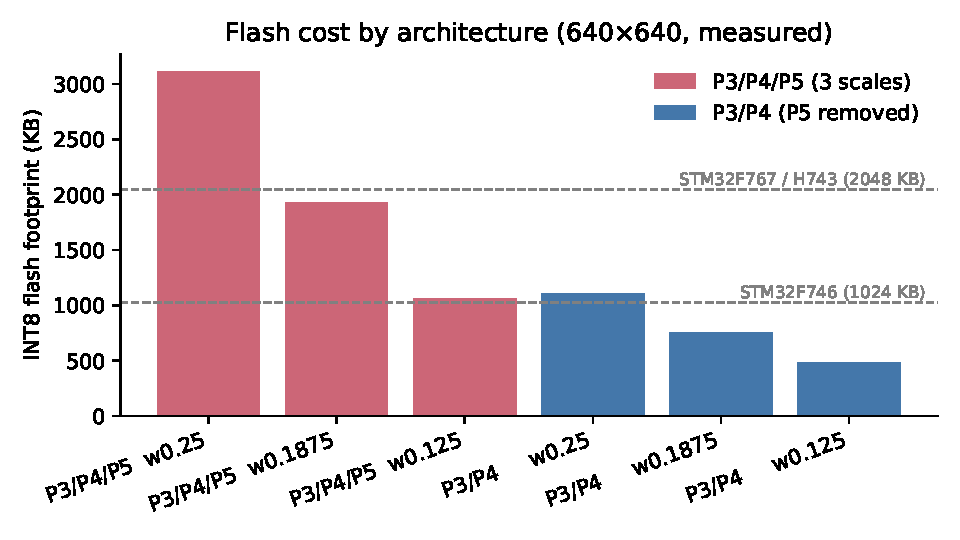
\includegraphics[width=0.75\textwidth]{figures/flash_by_variant.pdf}
\caption{INT8 flash footprint by architecture variant at
640$\times$640, against two plain-STM32 flash budgets. Removing the P5/32
pathway (blue) clears both reference lines that no three-scale variant
(red) reaches, even at the smallest width tested.}
\label{fig:flash-by-variant}
\end{figure}

The parameter count is not spread evenly across the stock network: the
P5/32 pathway (backbone stages 7--9 and the corresponding head stages)
accounts for 1{,}561{,}088 of 3{,}011{,}043 parameters (51.8\%); the
detection head for 751{,}507 (25.0\%); and the P3+P4 feature trunk for the
remaining 698{,}448 (23.2\%). Over half of the stock network exists to
detect objects large enough to be rare-to-absent in this deployment's
camera geometry (Section~\ref{sec:method-ablation}), and Table~\ref{tab:ablation-cost}
and Figure~\ref{fig:flash-by-variant} show that cutting it is the single
largest lever available on flash---larger than the INT8 step in
Table~\ref{tab:quant-tradeoff}, and the only lever, among those tested here,
that clears a plain-STM32 flash budget at 640$\times$640 at all.

The arena column in Table~\ref{tab:ablation-cost} tells an orthogonal story:
it barely moves across architectures. The peak sits at the very first
convolution in every variant---the input buffer
($3\times640\times640=1{,}200$ KB) plus that convolution's output
($16\times320\times320=1{,}600$ KB)---so \textbf{flash is set by
architecture, and activation RAM is set almost entirely by input
resolution.} No amount of architectural thinning touches it, because it is
set before the network has had a chance to downsample.

\subsection{Architecture ablation: trained accuracy}
\label{sec:ablation-accuracy}

\begin{table}[h]
\centering
\begin{tabular}{lcccccc}
\toprule
Variant & Epochs & mAP50 & mAP50-95 & Precision & Recall \\
\midrule
P3/P4/P5, $w$0.125 & 20 (patience 8, not triggered) & 0.9230 & 0.6886 & 0.9294 & 0.8673 \\
\textbf{P3/P4, $w$0.25} & 20 (patience 8, not triggered) & \textbf{0.9346} & \textbf{0.7216} & 0.9295 & 0.8718 \\
\bottomrule
\end{tabular}
\caption{Stage-2 trained comparison, both from random initialization, same
data and schedule. The two variants are matched to within 5.9\% of the same
parameter count and cost almost the same flash (Table~\ref{tab:ablation-cost}),
so this isolates a topology effect from a size effect.}
\label{tab:ablation-accuracy}
\end{table}

\begin{figure}[h]
\centering
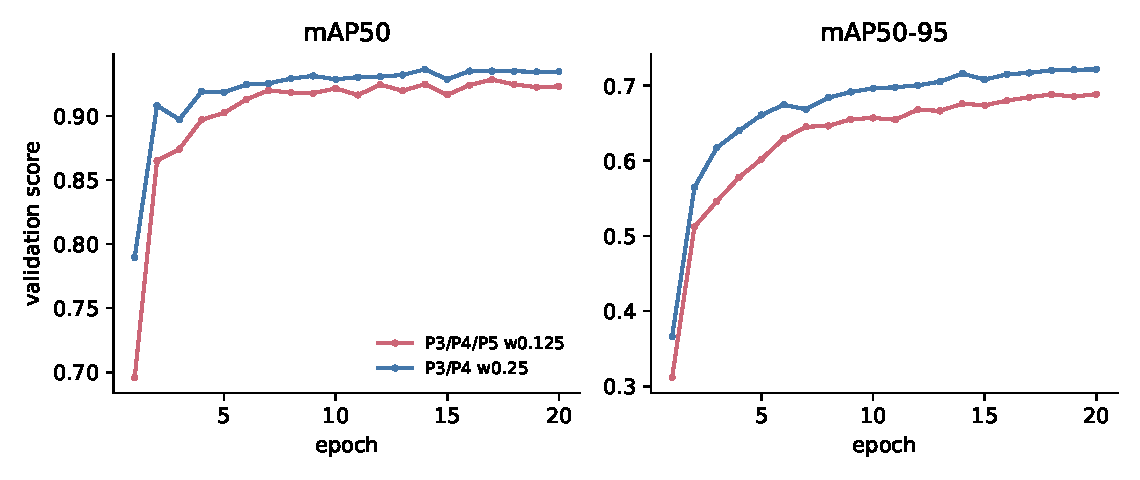
\includegraphics[width=0.95\textwidth]{figures/stage2_training_curves.pdf}
\caption{Validation mAP50 (left) and mAP50-95 (right) per epoch for both
Stage-2 finalists, trained from random initialization on identical data.
The two-scale, full-width variant (P3/P4, $w$0.25) is consistently above the
three-scale, thinned variant (P3/P4/P5, $w$0.125) across all 20 epochs on
both metrics.}
\label{fig:training-curves}
\end{figure}

At essentially matched parameter count and flash cost, the two-scale,
full-width architecture wins on every metric, most notably \textbf{+3.30
points of mAP50-95} (0.7216 vs.\ 0.6886). This confirms the hypothesis
motivating the ablation: the P5/32 capacity the stock network spends on
large-object detection is better spent as extra width on the two scales this
domain actually uses, rather than preserved (and thinned) across all three.
Figure~\ref{fig:training-curves} shows the gap is not a late-epoch artifact---
the full-width two-scale variant is ahead from early in training and the gap
is stable through all 20 epochs for both finalists (patience-8 early
stopping was not triggered by either run).

This win is not free. At matched flash, the two-scale full-width variant
needs 2{,}800 KB of activation arena against the three-scale thinned
variant's 2{,}000 KB---40\% more---because removing the P5 branch removes a
downsampling stage and leaves the widened P3/P4 branch doing its work at a
larger spatial resolution. On the most RAM-constrained deployment targets,
that 40\% can be the difference between fitting and not; see
Section~\ref{sec:deployment-envelope}.

Both results in this subsection, and only these two, are subject to the
single-run caveat in Section~\ref{sec:limitations}: each is one
random-initialization training run, with no repeated-seed variance estimate.

\section{Hardware Feasibility Discussion}
\label{sec:hw-feasibility}

\subsection{The stock architecture does not fit, at the native resolution}

Table~\ref{tab:feasibility-frontier} applies the stock architecture's
640$\times$640 footprint (Table~\ref{tab:ablation-cost}, baseline row) against
public datasheet budgets for four plain parts and two accelerator-equipped or
off-chip-memory parts.

\begin{table}[h]
\centering
\resizebox{\textwidth}{!}{%
\begin{tabular}{lccc}
\toprule
Target & Flash budget & RAM budget & Max workable input (stock arch.) \\
\midrule
STM32F746~\cite{stm32f7}        & 1 MB     & 320 KB  & none \\
STM32F767~\cite{stm32f7}        & 2 MB     & 512 KB  & none \\
STM32H743~\cite{stm32h7}        & 2 MB     & 1 MB    & none \\
ESP32-S3~\cite{esp32s3}         & 8 MB ext.\ flash & 512 KB & 256$\times$256 \\
ESP32-S3 + 8 MB PSRAM~\cite{esp32s3} & 8 MB ext.\ flash & 8 MB ext.\ PSRAM & 640$\times$640 \\
STM32N657 (NPU)~\cite{stm32n6}  & 8 MB ext.\ flash & 4.2 MB  & 640$\times$640 \\
\bottomrule
\end{tabular}%
}
\caption{Feasibility of the \emph{stock} architecture, swept over input
resolution, against each target's on-chip budget. None of the three plain
STM32 parts fit at any resolution; the three that do fit all rely on
off-chip memory, an accelerator, or both.}
\label{tab:feasibility-frontier}
\end{table}

Read honestly, the only rows that fit are the ones that change the rules:
the ESP32-S3 relies on \emph{external} flash and, past 256$\times$256,
external PSRAM, both off-chip and far slower than internal SRAM; the
STM32N657 fits comfortably, but it carries a Neural-ART neural accelerator---
precisely the class of dedicated AI silicon this paper set out to avoid
depending on. We keep it in the table deliberately, as a negative control:
it demonstrates the profiler correctly reports a positive result when one is
actually available, and it is the clearest illustration that the stock
architecture's problem is capacity, not an artifact of the measurement
method.

At this operating point, flash is the binding constraint: it overshoots the
largest plain part (STM32H743, 2,048 KB) by roughly 50\%, while the
640$\times$640 activation arena (2,800 KB, Table~\ref{tab:ablation-cost})
overshoots every plain part's RAM budget by an even larger margin---so
nothing in Table~\ref{tab:feasibility-frontier} depends on getting the
flash/RAM tradeoff exactly right; both constraints independently rule out
every plain part.

\subsection{Flash is architecture-bound; RAM is resolution-bound}

Section~\ref{sec:ablation-cost} already showed that cutting the P5/32
pathway moves flash by 2.8$\times$ while leaving the activation arena
essentially unchanged. The two constraints in
Table~\ref{tab:feasibility-frontier} therefore have \emph{different causes}
and need \emph{different levers}: flash is fixed by which weight tensors
exist (an architecture question, fixed at design time, independent of input
size), and activation RAM is fixed by the size of the input and the first
layer's output (a resolution question, independent of how many parameters
the rest of the network has). A deployment that only pulls one of these two
levers will stall on the other. Downscaling the input without also cutting
P5 fixes RAM but leaves flash at 3,117 KB, still over every plain budget.
Cutting P5 without downscaling the input fixes flash but leaves a
640$\times$640 arena of 2,800 KB, still over every plain budget except the
1 MB STM32H743. Both levers have to move together.

\subsection{The deployment envelope, pulling both levers}
\label{sec:deployment-envelope}

\begin{table}[h]
\centering
\begin{tabular}{lcccc}
\toprule
Target & Budget (flash / RAM) & Baseline & P3/P4, $w$0.25 & P3/P4, $w$0.125 \\
\midrule
STM32F746 & 1 MB / 320 KB & none & 192$\times$192 & 192$\times$192 \\
STM32F767 & 2 MB / 512 KB & none & 256$\times$256 & 256$\times$256 \\
STM32H743 & 2 MB / 1 MB   & none & \textbf{320$\times$320} & 416$\times$416 \\
\bottomrule
\end{tabular}
\caption{Largest input resolution that fits each plain target, by
architecture. Table~\ref{tab:feasibility-frontier}'s STM32H743 row read
``none''; with the P5-free architecture it reads 320$\times$320.}
\label{tab:deployment-envelope}
\end{table}

At the headline point---the two-scale, full-width architecture (the same one
that wins Section~\ref{sec:ablation-accuracy}'s trained comparison) at
320$\times$320 on an STM32H743---the requirement is 992.4 KB flash against a
2,048 KB budget, and 732.0 KB activation RAM against a 1,024 KB budget: both
roughly half the budget, leaving real room for the inference runtime and
application code that these figures exclude
(Section~\ref{sec:method-profiling}). The thinned three-scale variant
reaches a larger input (416$\times$416) on the same part, trading the
accuracy measured in Section~\ref{sec:ablation-accuracy} for headroom; which
of the two is the better deployment choice depends on whether the
application is more resolution-sensitive or accuracy-sensitive, a decision
this paper does not make on the deployer's behalf.

\subsection{Reconciling a stricter feasibility check at the native resolution}

The committed result artifact for this ablation also includes a stricter,
fixed-resolution feasibility check, evaluated only at
640$\times$640---the same resolution as Table~\ref{tab:feasibility-frontier}
---for all six Stage-1 variants, including the two-scale architectures. At
that fixed resolution, \emph{every} variant fails the RAM check on
\emph{every} plain target, including the two-scale architecture on the
STM32H743, because the 640$\times$640 activation arena (2,800 KB for the
two-scale, full-width variant; Table~\ref{tab:ablation-cost}) exceeds even
the H743's 1,024 KB budget on its own. This is not a contradiction of
Table~\ref{tab:deployment-envelope}: it is the same orthogonality result from
Section~5.2 stated the other way around. Table~\ref{tab:deployment-envelope}
answers ``what is the largest resolution that fits, letting resolution
vary''; the stricter check answers ``does the architecture fit at the input
size already fixed for the cost sweep''. Architecture alone was never going
to fix a RAM problem that is set by input resolution---downscaling to
320$\times$320 is the second, necessary lever, and Table~\ref{tab:deployment-envelope}
is the result of pulling it.

\section{Limitations and Future Work}
\label{sec:limitations}

\textbf{The headline mAP figures in this paper are self-referential and
should not be cited as detection-accuracy results.} As stated in
Section~2.1, ShanghaiTech ships only frame-level anomaly labels, not
bounding boxes. Training and validation labels for every fine-tuned model in
this paper were generated by running a COCO-pretrained YOLOv8n over the
dataset and keeping its own predictions as pseudo-labels; the fine-tuned
model was then scored against labels produced by a close relative of itself.
Every mAP figure in Tables~\ref{tab:quant-tradeoff}
and~\ref{tab:ablation-accuracy} therefore measures agreement with the base
model's own predictions on this footage, not ground-truth detection
accuracy, and the absolute values are inflated. This does not invalidate the
paper's central claims, because those claims are all \emph{relative}: the
INT8 accuracy cost (Table~\ref{tab:quant-tradeoff}) and the architecture
comparison (Table~\ref{tab:ablation-accuracy}) each hold the label set fixed
across every arm being compared, so the deltas are real even though the
absolute anchor is not. The one exception is
Table~\ref{tab:baseline-check}, scored against ShanghaiTech's genuine
human-authored labels---and even that result only certifies presence
detection, not localization quality. No subset of this dataset has been
hand-annotated with real bounding boxes; doing so (even a few hundred
frames) is the cheapest available fix if an absolute accuracy claim becomes
load-bearing later, and is listed as future work below.

Further limitations:

\begin{itemize}[leftmargin=1.4em, itemsep=0.2em]
  \item \textbf{Single run, no variance estimate.} Each Stage-2 architecture
  (Section~\ref{sec:ablation-accuracy}) was trained exactly once, from a
  single random initialization. The ranking is directional, not
  statistically certified; a seed-variance study would strengthen it.
  \item \textbf{Quantization-aware training was not pursued.} Post-training
  quantization's accuracy cost (0.2 points of mAP50) did not meet the bar
  set for escalating to QAT, which would add a full retraining cycle to
  recover a fraction of a point on an already self-referential metric. This
  was a deliberate scope decision, not an oversight.
  \item \textbf{MCU numbers are analytical, not vendor- or hardware-measured.}
  Section~\ref{sec:method-profiling}'s profiler was deliberately built to
  need no vendor account and no physical board, but STM32Cube.AI, Edge
  Impulse EON, or a flashed physical part would all likely report
  \emph{somewhat higher} figures (runtime overhead, buffer alignment,
  imperfect memory planning versus this paper's perfect-planner lower
  bound)---which would strengthen, not weaken, every negative result
  reported here, but has not been independently confirmed on real hardware.
  \item \textbf{No INT8 latency win was observed on CPU}
  (Section~\ref{sec:quant-results}), because general-purpose CPUs lack a
  fully optimized INT8 kernel path for this operator set. Whether INT8
  delivers the latency win on actual MCU-class cores with dedicated integer
  SIMD/DSP paths is untested here and is the more relevant question for the
  deployment target this paper argues for.
  \item \textbf{Dataset scale.} 28 scenes from a single campus, all
  fixed-mount, overhead-angle cameras. The P5/32-removal finding
  (Section~\ref{sec:ablation-cost}) is explicitly framed as a domain-specific
  trade conditioned on that camera geometry, not a general claim about
  YOLOv8 architecture.
\end{itemize}

\textbf{Future work:} validate the feasibility frontier
(Table~\ref{tab:deployment-envelope}) against a vendor toolchain and, ideally,
a physical STM32H743 board; hand-annotate a small ground-truth validation
subset to anchor the relative accuracy numbers to one honest absolute
figure; revisit QAT once an absolute accuracy anchor exists to measure it
against; repeat the Stage-2 training comparison across multiple seeds for a
variance estimate; measure INT8 latency on an actual MCU-class core; and
extend the pipeline to multi-camera re-identification, which the current
single-fixed-camera scope deliberately excludes.

\section{Conclusion}

Pushing person detection onto a plain microcontroller fails at the stock
architecture and succeeds after two changes that pull genuinely orthogonal
levers: removing a detection pathway the deployment's camera geometry never
exercises fixes flash, and downscaling the input fixes activation RAM.
Neither change alone is sufficient, and the architectural change additionally
turns out to be a free accuracy win, not just a compression trick, when
retrained from scratch and compared fairly against the alternative of
uniformly shrinking the stock network. The result is a detector that fits a
2016-era Cortex-M7 part with headroom to spare, with a deliberate
accelerator-equipped counterexample included specifically to show the
negative result elsewhere in this paper is a property of the problem, not a
limitation of the measurement.

\bibliographystyle{plain}
\bibliography{refs}

\end{document}
